
\subsubsection*{Estructuras del scheduler}
 
La estructura en la que almacenamos los datos necesarios para la conmutación de tareas es muy simple. Básicamente son 3 datos

\begin{lstlisting}
struct {
  uint indiceA;
  uint indiceB;

  cual_t proximo;
} sched_struct;
\end{lstlisting}


\texttt{indiceA} nos indica cual es el próximo índice en el que deberíamos comenzar a buscar una nueva tarea para ejecutar del jugador A (similarmente \texttt{indiceB}). Notar que este índice puede corresponderse con una tarea válida del jugador tanto como con una tarea muerta o inválida.
 
\texttt{proximo}, nos indica a que jugador le toca jugar, es decir, en que arreglo de tareas vamos a comenzar nuestra búsqueda.
 
\subsubsection*{Algoritmos del scheduler}
 
La estructura que elegimos para el scheduler se ve fuertemente reflejada en los algorimos. Primero notemos como inicializamos las estructuras, todas en 0, y elegimos, arbitrariamente, que el proximo jugador al que le tocará es el A (podríamos haber elegido obviamente cualquiera).
 
Ahora inspeccionamos la funcion \texttt{sched_proxima_a_ejecutar}. Lo que hace es muy simple. 
Si el jugador al que le toca jugar es el A, comenzara buscando por su arreglo, desde \texttt{indiceA}, algún pirata que este vivo, y en caso de encontrarlo hara 4 cosas: setear a B como el proximo jugador, setear la id de la tarea actual con el id de la tarea seleccionada, inicializar mineros del jugador, si es que había mineros pendientes y finalmente devolver el indice en la gdt de la tss de la tarea seleccionada.
En caso de no encontrarlo, hará exactamente lo mismo con el arreglo del jugador B, buscando piratas vivos y etc.
 
\subsubsection*{Interrupción de reloj}
 
La última parte del scheduler que nos toca analizar es la parte que hace la conmutación de tareas, que es la interrupción de reloj.
 
La rutina de atención de interrupción de reloj es muy similar a la que nos dieron en clase. La única diferencia que tiene es que se fija si está activada la pantalla de debug, y en ese caso no hace nada (dado que no queremos que mientras la pantalla de debug esté activada, los piratas se sigan moviendo por el mapa).
 
El comportamiento del resto es realmente simple, llamamos a la función que nos da el indice de la gdt de la tss de la proxima tarea a ejecutar, la comparamos en el índice de la tarea actual (si la tarea es la misma no debemos saltar, porque saltaríamos a una tarea que tiene el bit de Busy en 1 y explota todo) y en caso de que sea distintos, saltamos.
 
Es importante notar que cuando se le reasigne la ejecución a una tarea, esta tarea va a volver a la linea que dice \texttt{popfd} y luego volverá a su ejecución común y corriente.
 
\subsubsection*{Modo Debug}
 
El modo debug es fácil de hacer una vez que el resto de las cosas están bien hechas. Debimos agregar un par de variables globales que nos indiquen si el modo debug está activado y otra que nos indique si se está mostrando la pantalla de debug en un momento dado.
 
Cuando nos llega una interrupción de las primeras 20, lo que hacemos es guardar toda la información que este disponible en ese momento (la que debemos guardar) y luego llamar a \texttt{game_pirata_exploto}.
 
En \texttt{game_pirata_exploto} (ademas de hacer las limpiezas de estructuras que correspondan) lo que hacemos es chequ si está el modo debug activado o no. En caso afirmativo, cargamos ciertas cosas que sean necesarias y llamamos a la función \texttt{screen_debug} que es realmente simple, muestra todos los datos en pantalla, mientras siga activado el modo debug. Cuando se vuelve a apretar 'y', el modo debug se desactiva y se sale de el loop, restaurando la pantalla como estaba (que previamente había sido backupeada).
 
\begin{figure}[ht!]
\centering
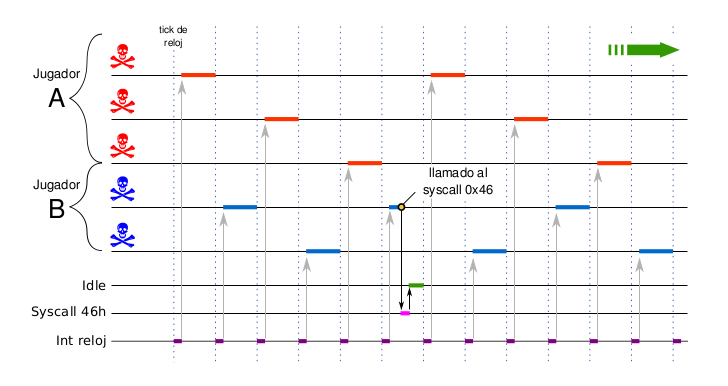
\includegraphics[width=100mm]{imagenes/scheduler.png}
\caption{Funcionamiento del Scheduler}
\end{figure}

